\section{Analisis dan Rancangan Solusi}

Berdasarkan analisis masalah, terdapat beberapa solusi yang dapat langsung menjawab permasalahan yang diuraikan pada Bab \ref{sec:analisis-persoalan}. Pemetaan analisis dan rancangan solusi terhadap analisis masalah terdapat dalam tabel berikut.

\begin{table}[h!]
    \centering
    \begin{tabular}{|m{0.45\linewidth}|m{0.45\linewidth}|}
    \hline
    \rowcolor{black!10}
    \textbf{Analisis Masalah} & \textbf{Analisis dan Rancangan Solusi} \\ \hline
    (1) Kakas IndoLEM yang \textit{outdated} & (1) Refaktorisasi kakas IndoLEM \\ \hline
    (2) Pengembangan metode PETL pada kakas IndoLEM & (2) Mengembangkan setiap metode PETL pada kakas IndoLEM \\ \hline
    (3) Pemilihan konfigurasi terbaik untuk setiap metode PETL & (3) Eksperimen terhadap berbagai konfigurasi metode PETL \\ \hline
    (4) Pemilihan kombinasi \textit{hyperparameter} terbaik pada proses \textit{training} & (4) Penelusuran kombinasi \textit{hyperparameter} terbaik\\ \hline
    (5) Pemilihan metode evaluasi & (5) Penelusuran metode evaluasi yang relevan \\ \hline
    \end{tabular}
\caption{Pemetaan analisis dan rancangan solusi terhadap analisis masalah}
\label{table:pemetaan-masalah-solusi}
\end{table}

Berdasarkan analisis solusi terhadap setiap analisis masalah yang terdapat pada tabel \ref{table:pemetaan-masalah-solusi}, dibangun sebuah rancangan solusi berupa skenario pengujian yang dilakukan dalam penelitian tugas akhir, yang dapat dilihat pada Gambar \ref{fig:rancangan-solusi}. Berdasarkan Gambar \ref{fig:rancangan-solusi}, tidak ditambahkan dataset baru, melainkan menggunakan dataset yang sudah disediakan pada IndoLEM. Teknik PETL yang digunakan adalah LoRA (\textit{Low-Rank Adaptation}), \textit{Prefix-Tuning}, dan \textit{Tiny-Attention Adapter}. Hasil pengujian berupa kinerja dari teknik PETL serta penggunaan sumber daya dari setiap eksperimen.

\begin{figure}[ht]
    \centering
    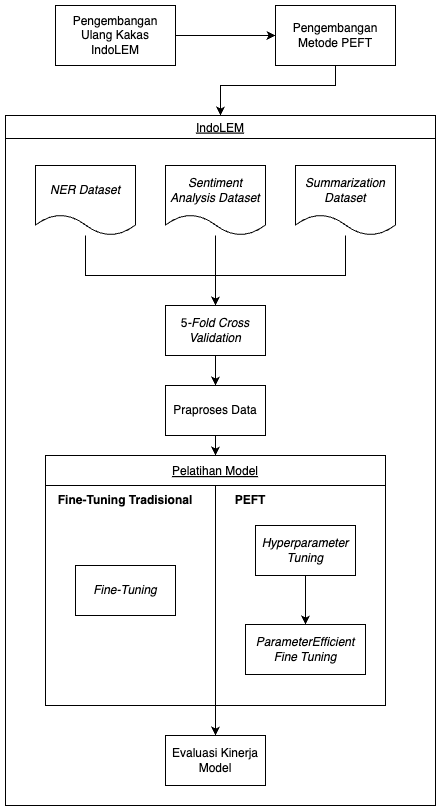
\includegraphics[width=1\textwidth]{chapter-3/rancangan_solusi.png}
    \caption{Rancangan Solusi}
    \label{fig:rancangan-solusi}
\end{figure}
